\documentclass[conference,a4paper]{IEEEtran}
\pdfminorversion=6
\usepackage{amsmath,amssymb}
\usepackage{graphicx}
\usepackage{booktabs}
\usepackage{array}
\usepackage{url}
\usepackage{cite}

\begin{document}

\title{Efficient Visualization of Knowledge Bases via Space-Time Graphs:\\ The OHARA Architecture}

\author{
\IEEEauthorblockN{Thanh-Tung Pham}
\IEEEauthorblockA{University of Science, Vietnam National University -- Ho Chi Minh City\\ pttung@fit.hcmus.edu.vn}
}

\maketitle

\begin{abstract}
Flat-chunk retrieval-augmented generation (RAG) returns ranked lists that give users no spatial or temporal model of a growing corpus. We present OHARA, an architecture built on a \emph{Space-Time Graph} that unifies document structural hierarchy, temporal decay, and cross-document entity/ontology pivots as a single substrate for both retrieval and a novel 3D sunburst-tunnel visualization (time $\to$ Z-axis, ontology $\to$ sunburst cross-section, document structure $\to$ radial discs). An eight-phase hybrid retrieval engine fuses lexical, dense, ontology, entity, structural, and cross-document signals into tiered, provenance-carrying results. On two corpora (QASPER-200 academic papers, MultiHop-RAG-609 news articles) the tuned fusion pipeline reaches ranking \emph{parity} with the best single dense signal, not superiority; the differentiated, quantitatively supported result is a corroboration-gated Principal tier that abstains on 45.6\% of unanswerable queries versus 0.0\% for a plain top-$k$ cut, at 91.5\% Principal-hit on answerable queries. Ingest builds the full semantic graph at roughly \$12 per 1{,}000 documents; the visualization renders sub-linearly to 12{,}323 nodes. We report these results honestly, including a negative finding on temporal decay scoring, and frame OHARA's contribution as a knowledge base that is \emph{seeable and auditable} rather than one that outranks dense retrieval.
\end{abstract}

\begin{IEEEkeywords}
retrieval-augmented generation, knowledge graph, information visualization, ontology, temporal reasoning
\end{IEEEkeywords}

\section{Introduction}

Flat-chunk RAG pipelines return a linear list of passages; users lose the spatial or temporal context of where each passage sits in the corpus, compounding the ``lost in the middle'' effect of long contexts \cite{liu2024lost}. Retrieval-augmented generation has matured into a broad architectural space \cite{gao2023ragsurvey}, with graph-structured variants now surveyed as their own subfield \cite{peng2024graphrag_survey}. OHARA targets corpora that carry, or can be given, structural metadata (sections, paragraphs, tables) and publication dates -- regulatory filings, academic papers, technical manuals, long-form journalism.

\textbf{Contributions.} (a) An efficient 3D sunburst-tunnel visualization mapping time to the Z-axis, ontology to a sunburst polar plane, document structure to radial discs, and decay class to a temporal-reach aura. (b) A Space-Time Graph data model combining structural hierarchy, temporal decay, and cross-document entity pivots, serving as both retrieval substrate and visualization coordinate system. (c) A multi-phase hybrid retrieval engine whose measured value is tiered, provenance-carrying results at parity with the best single-signal retriever, not ranking gains. (d) A corroboration-gated Principal tier that abstains on unanswerable queries where a top-$k$ cut structurally cannot -- at identical retrieval, the $\geq$2-signal gate abstains on 45.6\% of MultiHop-RAG null queries versus 0.0\% for plain top-$k$, holding 91.5\% Principal-hit on answerable queries. (e) A SUMO ontology-grounded semantic layer that anchors the visualization's coordinates and enables tag-expansion retrieval.

We state our positioning explicitly: OHARA does not claim graph-augmented retrieval outranks dense retrieval -- our evaluation (Sec.~\ref{sec:eval}) shows the tuned hybrid \emph{matches} the best single signal. The thesis is that a knowledge base should be seeable and auditable: the same graph that answers a query renders as a navigable spatial-temporal map and attaches per-result provenance, abstaining rather than emitting $k$ confident-looking passages when nothing is corroborated.

\section{Related Work}

Graph-based RAG systems (GraphRAG \cite{edge2024graphrag}, LightRAG \cite{guo2024lightrag}, HippoRAG \cite{gutierrez2024hipporag}) build entity/relation subgraphs but discard document structural hierarchy and couple retrieval to no temporal or spatial model. Explainable-retrieval work (Self-RAG \cite{asai2023selfrag}, Corrective RAG \cite{yan2024crag}) targets provenance but not 3D navigation. Prior 3D and temporal graph visualizations (Time-arc, Storyline, VR graph tools) do not combine an ontology sunburst cross-section with a temporal tunnel axis; OHARA's layout builds on the 2D radial space-filling hierarchy tradition \cite{stasko2000focus} extended into a temporal third dimension so topic columns remain traceable through time. Table~\ref{tab:related} summarizes the gap: no compared system combines structural hierarchy, SUMO ontology grounding, temporal decay, and tiered explainability.

\begin{table}[t]
\centering
\caption{Capability comparison against graph-RAG baselines.}
\label{tab:related}
\scriptsize
\setlength{\tabcolsep}{2.5pt}
\begin{tabular}{lcccc}
\toprule
Capability & GraphRAG & LightRAG & HippoRAG & OHARA \\
\midrule
Entity/relation subgraph & \checkmark & \checkmark & \checkmark & \checkmark \\
Structural hierarchy (DoCO) & -- & -- & -- & \checkmark \\
Cross-doc similarity edges & partial & \checkmark & \checkmark & \checkmark \\
SUMO ontology grounding & -- & -- & -- & \checkmark \\
Temporal decay scoring & -- & -- & -- & \checkmark \\
3D space-time visualization & -- & -- & -- & \checkmark \\
Tiered explainability & -- & -- & -- & \checkmark \\
\bottomrule
\end{tabular}
\end{table}

\section{The Space-Time Graph Data Model}

The Space-Time Graph is a 5-tuple $G = (V, E, \tau, \delta, \sigma)$. The vertex set $V = V_{docs} \cup V_{sect} \cup V_{para} \cup V_{tab} \cup V_{ent}$ spans document roots, structural hierarchy nodes, content nodes (paragraphs/tables), and named entities. Edges $E \subseteq V \times V \times R$ are typed by seven relations
\begin{equation*}
\small
R = \{\textsc{has\_child}, \textsc{next\_sibling}, \textsc{belongs\_to}, \textsc{mentions},
\end{equation*}
\begin{equation*}
\small
\textsc{related\_to}, \textsc{similar\_to}, \textsc{toc\_ref}\},
\end{equation*}
spanning structural (tree), semantic (cross-cutting), and cross-document (Jaccard-gated) relationships. Temporal bucketing $\tau: V_{docs} \to \Theta$ maps documents to a Z-axis coordinate at configurable resolution; decay classification $\delta: V_{docs} \to D$ assigns one of four classes (\textsc{evergreen} $\lambda{=}10^{-6}$, \textsc{scholarly} $\lambda{=}10^{-4}$, \textsc{current} $\lambda{=}10^{-2}$, \textsc{ephemeral} $\lambda{=}10^{-1}$), auto-promoted to \textsc{evergreen} when in-degree of \textsc{similar\_to} $\geq 5$; narrative enrichment $\sigma$ attaches a verb, tags, summary, and temporal relation to cross-document edges. Decay scoring uses $w \cdot e^{-\lambda \Delta t}$ under a five-layer protection scheme (no temporal intent, Principal-tier immunity, high-BM25 immunity, weak-candidate-only, and date-range coverage boost) that we present as a guard-railed recency prior rather than a demonstrated ranking gain: on the one temporal benchmark evaluated the prior is neutral-to-slightly-negative (Sec.~\ref{sec:eval}, finding 3), with genuine freshness domains (news monitoring, versioned documentation) left as future validation.

\textbf{Pre-filtering complexity.} At ingest, each document's paragraph-level \texttt{entity\_slugs} and \texttt{sumo\_tags} are unioned onto its root node (document rollup). Query-time candidate pruning then scans $O(n)$ document rollups, $n = |V_{docs}|$, instead of $O(n \times \text{chunks\_per\_doc})$ content nodes -- a $\sim$50--60$\times$ reduction at our measured corpus densities (16 sections, 44 paragraphs per document). Whether the subsequent \emph{descent} into the pruned document finds the correct paragraph is the empirical bottleneck, not the pre-filter's cost: our evaluation attributes $\sim$42\% of corpus-wide retrieval failures to document location and descent (Sec.~\ref{sec:eval71}).

\section{Multi-Phase Hybrid Retrieval Engine}

Eight signal phases run in a configurable pipeline: (0) query fingerprinting -- keyword/phrase/paragraph classification with Gemini-extracted SUMO tags, entity hints, and temporal intent for phrase-length queries and above; (0b) TOC-guided section selection, an LLM pass over seed document tables of contents that supplies structural traversal entry points; (1) BM25 full-text; (1b) SUMO tag overlap with hierarchy expansion; (1c) multi-hop \textsc{similar\_to} traversal carrying narrative edge verbs and summaries; (1d) dense vector similarity (\texttt{gemini-embedding-2}, 768-d, cosine); (2) entity pivot across shared canonical entities; (3) structural traversal (depth 2) with a corrective filter dropping zero-SUMO-overlap nodes. Phase 4 fuses per-phase max-normalized scores with a weighted sum (base weights BM25 1.0, vector 0.5, SUMO 0.4, entity 0.6, cross-doc 0.4, structural 0.3, scaled by query-mode multipliers) and adds the guarded temporal contribution.

\textbf{Tier classification.} Grounded in Bates' Berrypicking and Pirolli's Information Foraging Theory: \emph{Principal} nodes require $\geq$2 independent phase contributions, cross-document or multi-document evidence, and score above the 75th percentile; \emph{Integrity} adds verified structural and cross-document neighbors; \emph{Explorer} is a metadata-only frontier one hop beyond Integrity, filtered to a weakening-scent weight band. In practice the corroborating pair for Principal-tier membership is almost always \texttt{bm25}$\cap$\texttt{vector} -- the graph-side phases (entity, cross-document, structural) exclude already-seen nodes by design and so expand the frontier rather than corroborate the core. This constraint's quantitatively confirmed payoff is abstention, not ranking (Sec.~\ref{sec:eval}, finding 2): a top-$k$ cut cannot express ``no confident answer,'' while the $\geq$2-signal Principal gate can and does.

\section{Ingest Pipeline}

Parsing (LiteParse for PDF/EPUB/DOCX, Markdown pass-through) is followed by content-hash-cached LLM structuring into DoCO node types (\texttt{gemini-2.5-flash-lite}, concurrency 4), three-stage SUMO tag validation against a 22{,}700-entry index (exact, case-insensitive, alias table), entity extraction with canonical cross-document deduplication, structural/semantic edge creation with document rollup, and Jaccard-gated cross-document similarity enriched with an LLM-generated verb, tag set, summary, and temporal relation per edge. Measured at scale, ingesting 200 QASPER papers consumed 6.2M prompt + 4.5M output tokens ($\sim$53k/doc), \$2.41 at standard rates ($\sim$\$1.20 flex tier) -- roughly \$12 per 1{,}000 documents for the full semantic graph. Content-hash caching makes idempotent re-ingest near-free: 14.5\% of documents suffered a transient API failure on first pass, all recovered at near-zero marginal cost. One caveat: forced re-ingest of partial documents duplicated structural edges (23k duplicates across 13k pairs), so ingest idempotency currently holds at chunk level, not edge level.

\section{Space-Time Graph Visualization}

The visualization rests on three irreducible dimensions no 2D projection preserves simultaneously: time, ontology, and structure. The Z-axis carries resolution-bucketed publication time; the XY cross-section is an ontology sunburst plane in which each document sits at the polar coordinate of its top SUMO category ($\theta$ from a precomputed recursive angular partition of the SUMO tree, $r = R_{max}\sqrt{depth/D_{max}}$), so documents sharing a category stack into a stable topic column traceable along Z. Each document unfolds locally as a disc perpendicular to Z: the document node at center, section nodes in concentric rings by hierarchy level, paragraphs and tables on the outermost ring (Fig.~\ref{fig:viz}). Named entities sit at the centroid of the documents that mention them, pushed outward by a fixed offset; semi-transparent decay-class auras (5/2.5/1/0.4 disc-spans for \textsc{evergreen}/\textsc{scholarly}/\textsc{current}/\textsc{ephemeral}) make temporal reach spatially legible even where decay does not help ranking. Rendering uses Three.js \texttt{InstancedMesh} batching (one draw call per shape bucket) with lazy per-document, per-node loading. Measured on QASPER (headless Chromium, software WebGL, a conservative lower bound): scene rebuild and JS heap grow sub-linearly from 713 to 12{,}323 nodes (1.5\,s$\to$2.3\,s rebuild, 52\,MB$\to$80\,MB heap, a 17$\times$ node increase yielding only $\sim$1.7$\times$/$\sim$1.5$\times$ growth), confirming the practical ceiling is visual clutter and fill-rate, not geometry submission. A within-subjects user study protocol (flat list vs.\ sunburst-tunnel, $n\geq8$, temporal filtering / topic tracing / structural lookup tasks) is fully specified but not yet run. Fig.~\ref{fig:ui} shows the live application: a corpus-scale tunnel view and a drill-down into one document's disc with inline text inspection.

\begin{figure}[t]
\centering
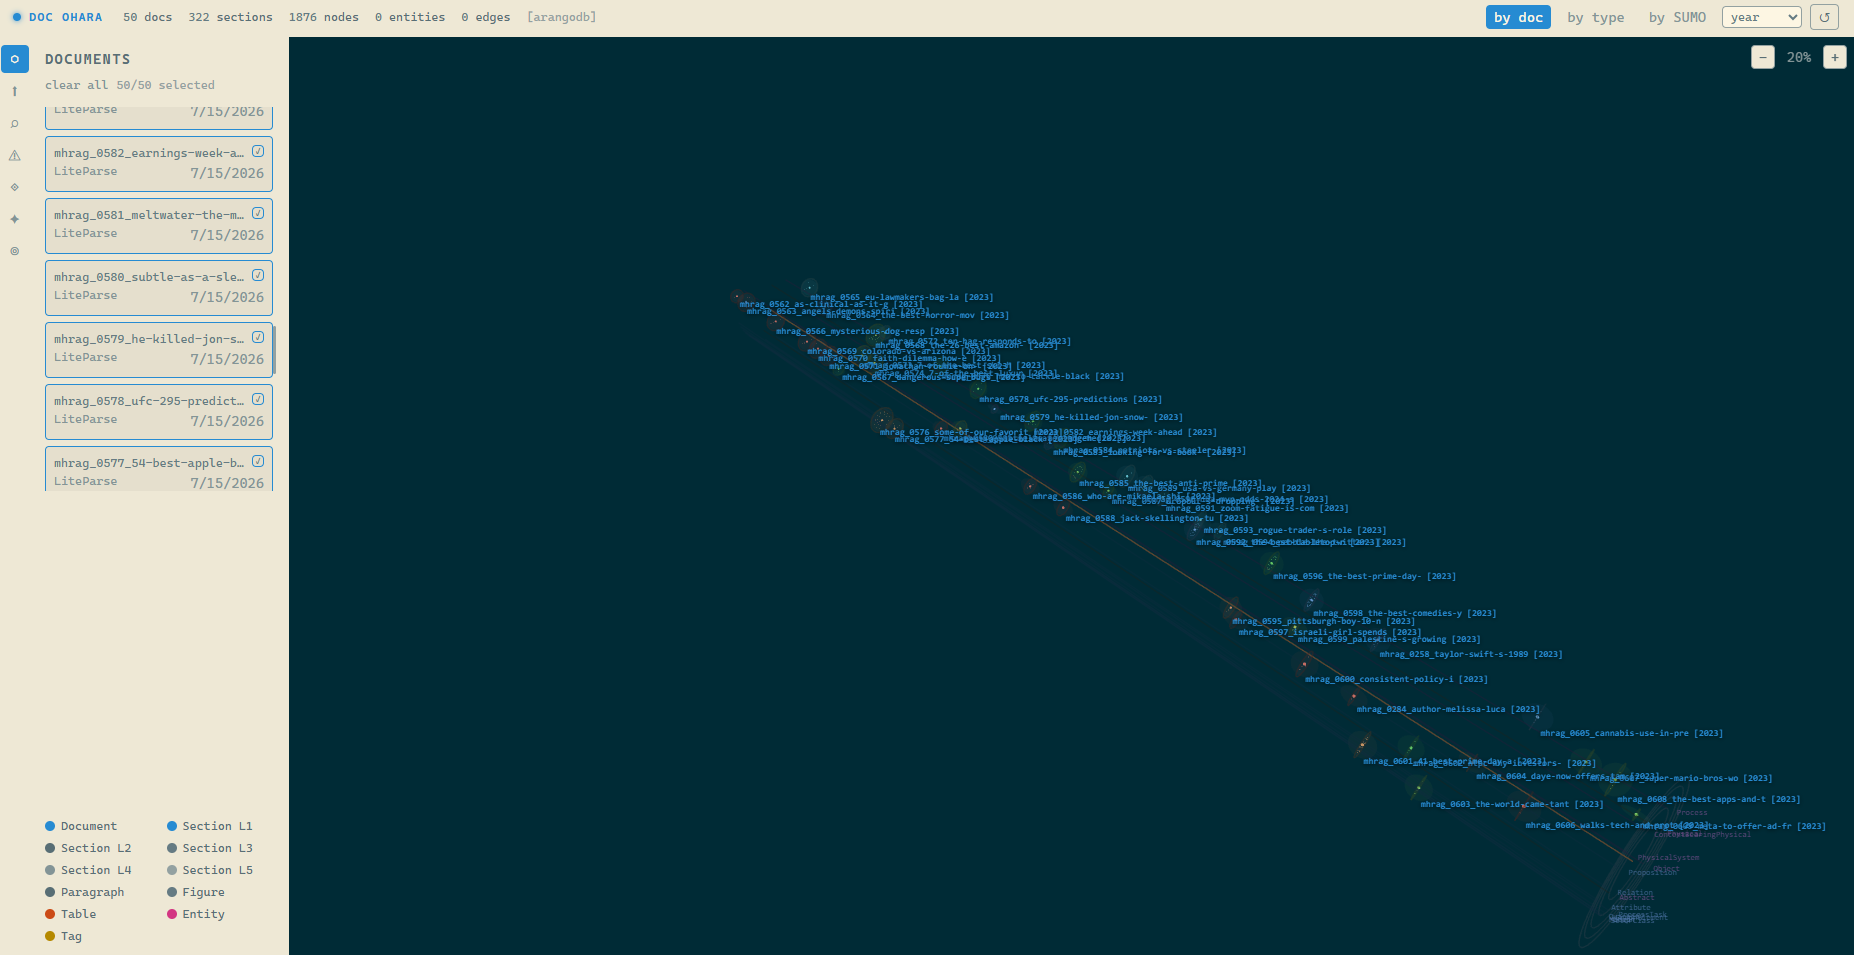
\includegraphics[width=\columnwidth]{figs/ui_overview.png}
\\[4pt]
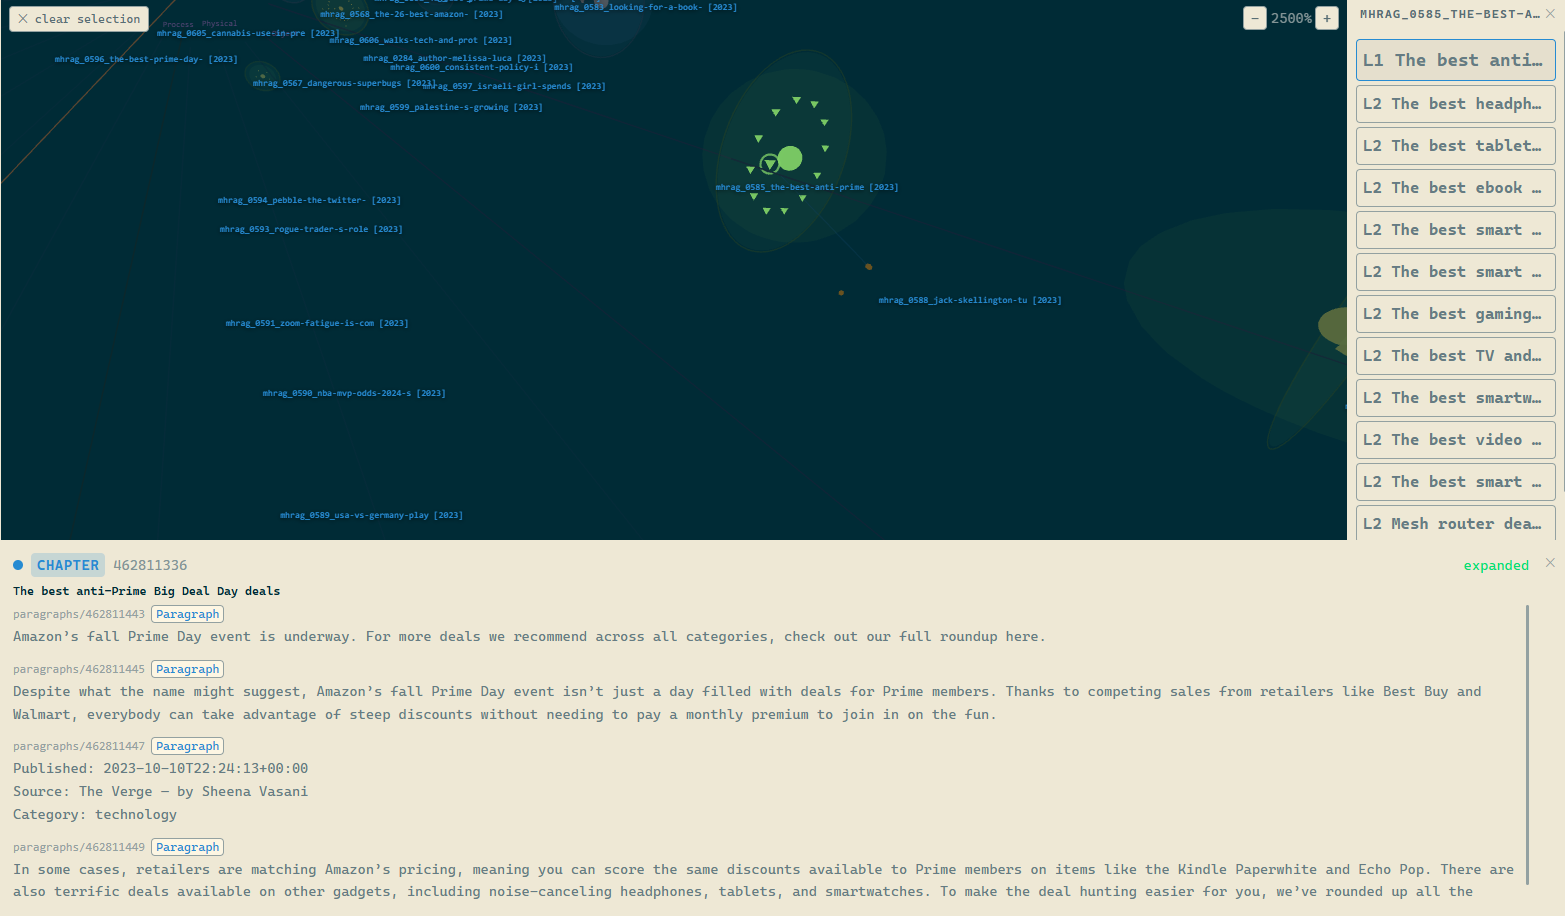
\includegraphics[width=\columnwidth]{figs/ui_detail.png}
\caption{The interactive application. \emph{Top}: full tunnel view at year resolution, 50 documents, colored by document -- sidebar lists selected documents and the node-type legend, header shows live corpus stats and view-mode toggles. \emph{Bottom}: zoomed into a single document's disc with a paragraph node selected, opening the right-hand inspector panel with the section outline and full extracted text/metadata (published date, source, category).}
\label{fig:ui}
\end{figure}

\section{Evaluation}
\label{sec:eval}

We evaluate on two corpora: QASPER (200 academic papers, 150 answerable questions, paragraph-level gold, scored corpus-wide over 229 documents including distractors) and MultiHop-RAG (609 news articles, 500 stratified queries including 125 null/unanswerable, document-level gold). A preliminary smoke run surfaced two silent failure modes fixed before the reported runs: raw BM25 magnitudes ($\sim$13--24) dominating bounded phase contributions absent per-phase normalization, and a stored/query-side embedding-model mismatch; both are corrected in all figures below.

\subsection{QASPER Retrieval Quality}
\label{sec:eval71}

Table~\ref{tab:qasper} reports the headline configurations. BM25-only badly underperforms vector-only (25.3\% vs.\ 33.3\% Hits@10) because corpus-wide lexical overlap collides across 229 documents -- the inverse of BM25's role \emph{within} one paper, where it is the strongest signal. The default-weight full pipeline (30.0\% Hits@10) trails vector-only because BM25 at weight 1.0 ranks lexical noise above semantic hits on this paraphrase-heavy benchmark; a grid search over (BM25, vector) weights on a held-out subset selects (0.6, 1.0), which recovers the gap entirely and slightly exceeds vector-only on MRR (0.179 vs.\ 0.175). Decomposing failures against an oracle that ranks only within the gold document shows corpus-wide loss concentrates in document \emph{location}: $\sim$42\% of queries fail before the correct document is even reached, while paragraph discrimination given the correct document succeeds for roughly two-thirds of queries (oracle Hits@10 64.4\%, in the band of published within-document baselines).

\begin{table}[t]
\centering
\caption{QASPER retrieval quality (150 questions, corpus-wide over 229 docs).}
\label{tab:qasper}
\scriptsize
\setlength{\tabcolsep}{3pt}
\begin{tabular}{lcccc}
\toprule
Config & H@4 & H@10 & MRR@10 & P-hit \\
\midrule
BM25-only & 12.7\% & 25.3\% & 0.102 & 0.0\% \\
Vector-only & \textbf{26.7\%} & \textbf{33.3\%} & 0.175 & \textbf{24.7\%} \\
Full (default) & 22.0\% & 30.0\% & 0.164 & 22.7\% \\
Full (tuned) & 25.3\% & \textbf{33.3\%} & \textbf{0.179} & 22.7\% \\
\bottomrule
\end{tabular}
\end{table}

\subsection{MultiHop-RAG Retrieval Quality and Abstention}

The QASPER-tuned weights (0.6, 1.0) transfer unchanged to MultiHop-RAG (Table~\ref{tab:multihop}), reaching Hits@10/MRR parity with vector-only while exceeding it on MAP (0.556 vs.\ 0.538). Three findings decide the paper's central claims. \textbf{First}, weight transfer generalizes: the lexical-first \emph{default} prior, not the fusion architecture, was the gap on both corpora. \textbf{Second}, corroboration-gated abstention is the one differentiated quantitative win: comparing full vs.\ the same pipeline with the corroboration constraint removed (identical retrieval, differing only in the tier rule) shows the constrained Principal tier abstains on 45.6\% of unanswerable queries versus 0.0\% for a plain top-$k$ cut, at 91.5\% Principal-hit on answerable queries; tuning trades some of this away (31.2\%) as an explicit precision/abstention trade-off. \textbf{Third}, temporal decay is an honest negative here: removing it \emph{improves} MRR on the temporal query slice (0.749 vs.\ 0.736), because MultiHop-RAG's temporal queries test event ordering, not recency, and the guard layers bound the resulting damage to $\sim$1pp. Per-phase ablations on both corpora land within $\pm$0.5pp of the full pipeline -- graph phases (SUMO, cross-document, structural, TOC) contribute provenance and abstention, not ranking lift, on the corpora tested. An end-to-end generation check (top-10 context, \texttt{gemini-2.5-flash-lite}) shows 54\% (tuned) vs.\ 57\% (vector-only) accuracy, mirroring retrieval parity; the dominant failure (41\%) is insufficient retrieved context, not hallucination.

\begin{table}[t]
\centering
\caption{MultiHop-RAG retrieval quality (500 stratified queries).}
\label{tab:multihop}
\scriptsize
\setlength{\tabcolsep}{3pt}
\begin{tabular}{lcccc}
\toprule
Config & H@10 & MRR@10 & P-hit & Null abst. \\
\midrule
BM25-only & 94.4\% & 0.727 & 4.3\% & 96.8\%* \\
Vector-only & \textbf{98.4\%} & 0.811 & \textbf{92.5\%} & 13.6\% \\
Full (default) & 96.5\% & 0.791 & 91.5\% & \textbf{45.6\%} \\
$-$ Corrob. & 96.8\% & 0.795 & 92.0\%† & 0.0\% \\
Full (tuned) & \textbf{98.4\%} & \textbf{0.812} & 92.0\% & 31.2\% \\
\bottomrule
\end{tabular}
\vspace{2pt}
\footnotesize{*Degenerate: near-empty Principal tier, not discrimination. †Proxied as top-5.}
\end{table}

\section{Discussion}

\textbf{Limitations.} Single LLM backend (Gemini) throughout structuring, tagging, and enrichment. Both evaluation corpora are clean born-digital text; noisy OCR and non-English corpora are untested. Fusion weights were tuned on one QASPER subset and, while shown to transfer to MultiHop-RAG, two corpora do not establish domain-general defaults. Visualization rendering is validated to 12k nodes but grows visually cluttered past $\sim$50 selected documents; the user study protocol is prepared but not yet run.

\textbf{Research agenda.} We separate measured results from open hypotheses. (H1) Ranking gains from spatial-temporal structure: today's parity result caps corroboration at two signal families because graph phases exclude already-seen nodes; letting them re-score seen nodes to enable many-angle corroboration is the direct next experiment. (H2) Recency-semantic temporal scoring: today's result is neutral-to-negative on event-ordering queries; corpora with genuine freshness semantics (news monitoring, versioned documentation) remain untested. (H3) The human navigation benefit of the 3D spatial-temporal mental model is the thesis claim, untested by the scope of this paper, with protocol and rendering substrate both validated and ready.

\begin{figure}[t]
\centering
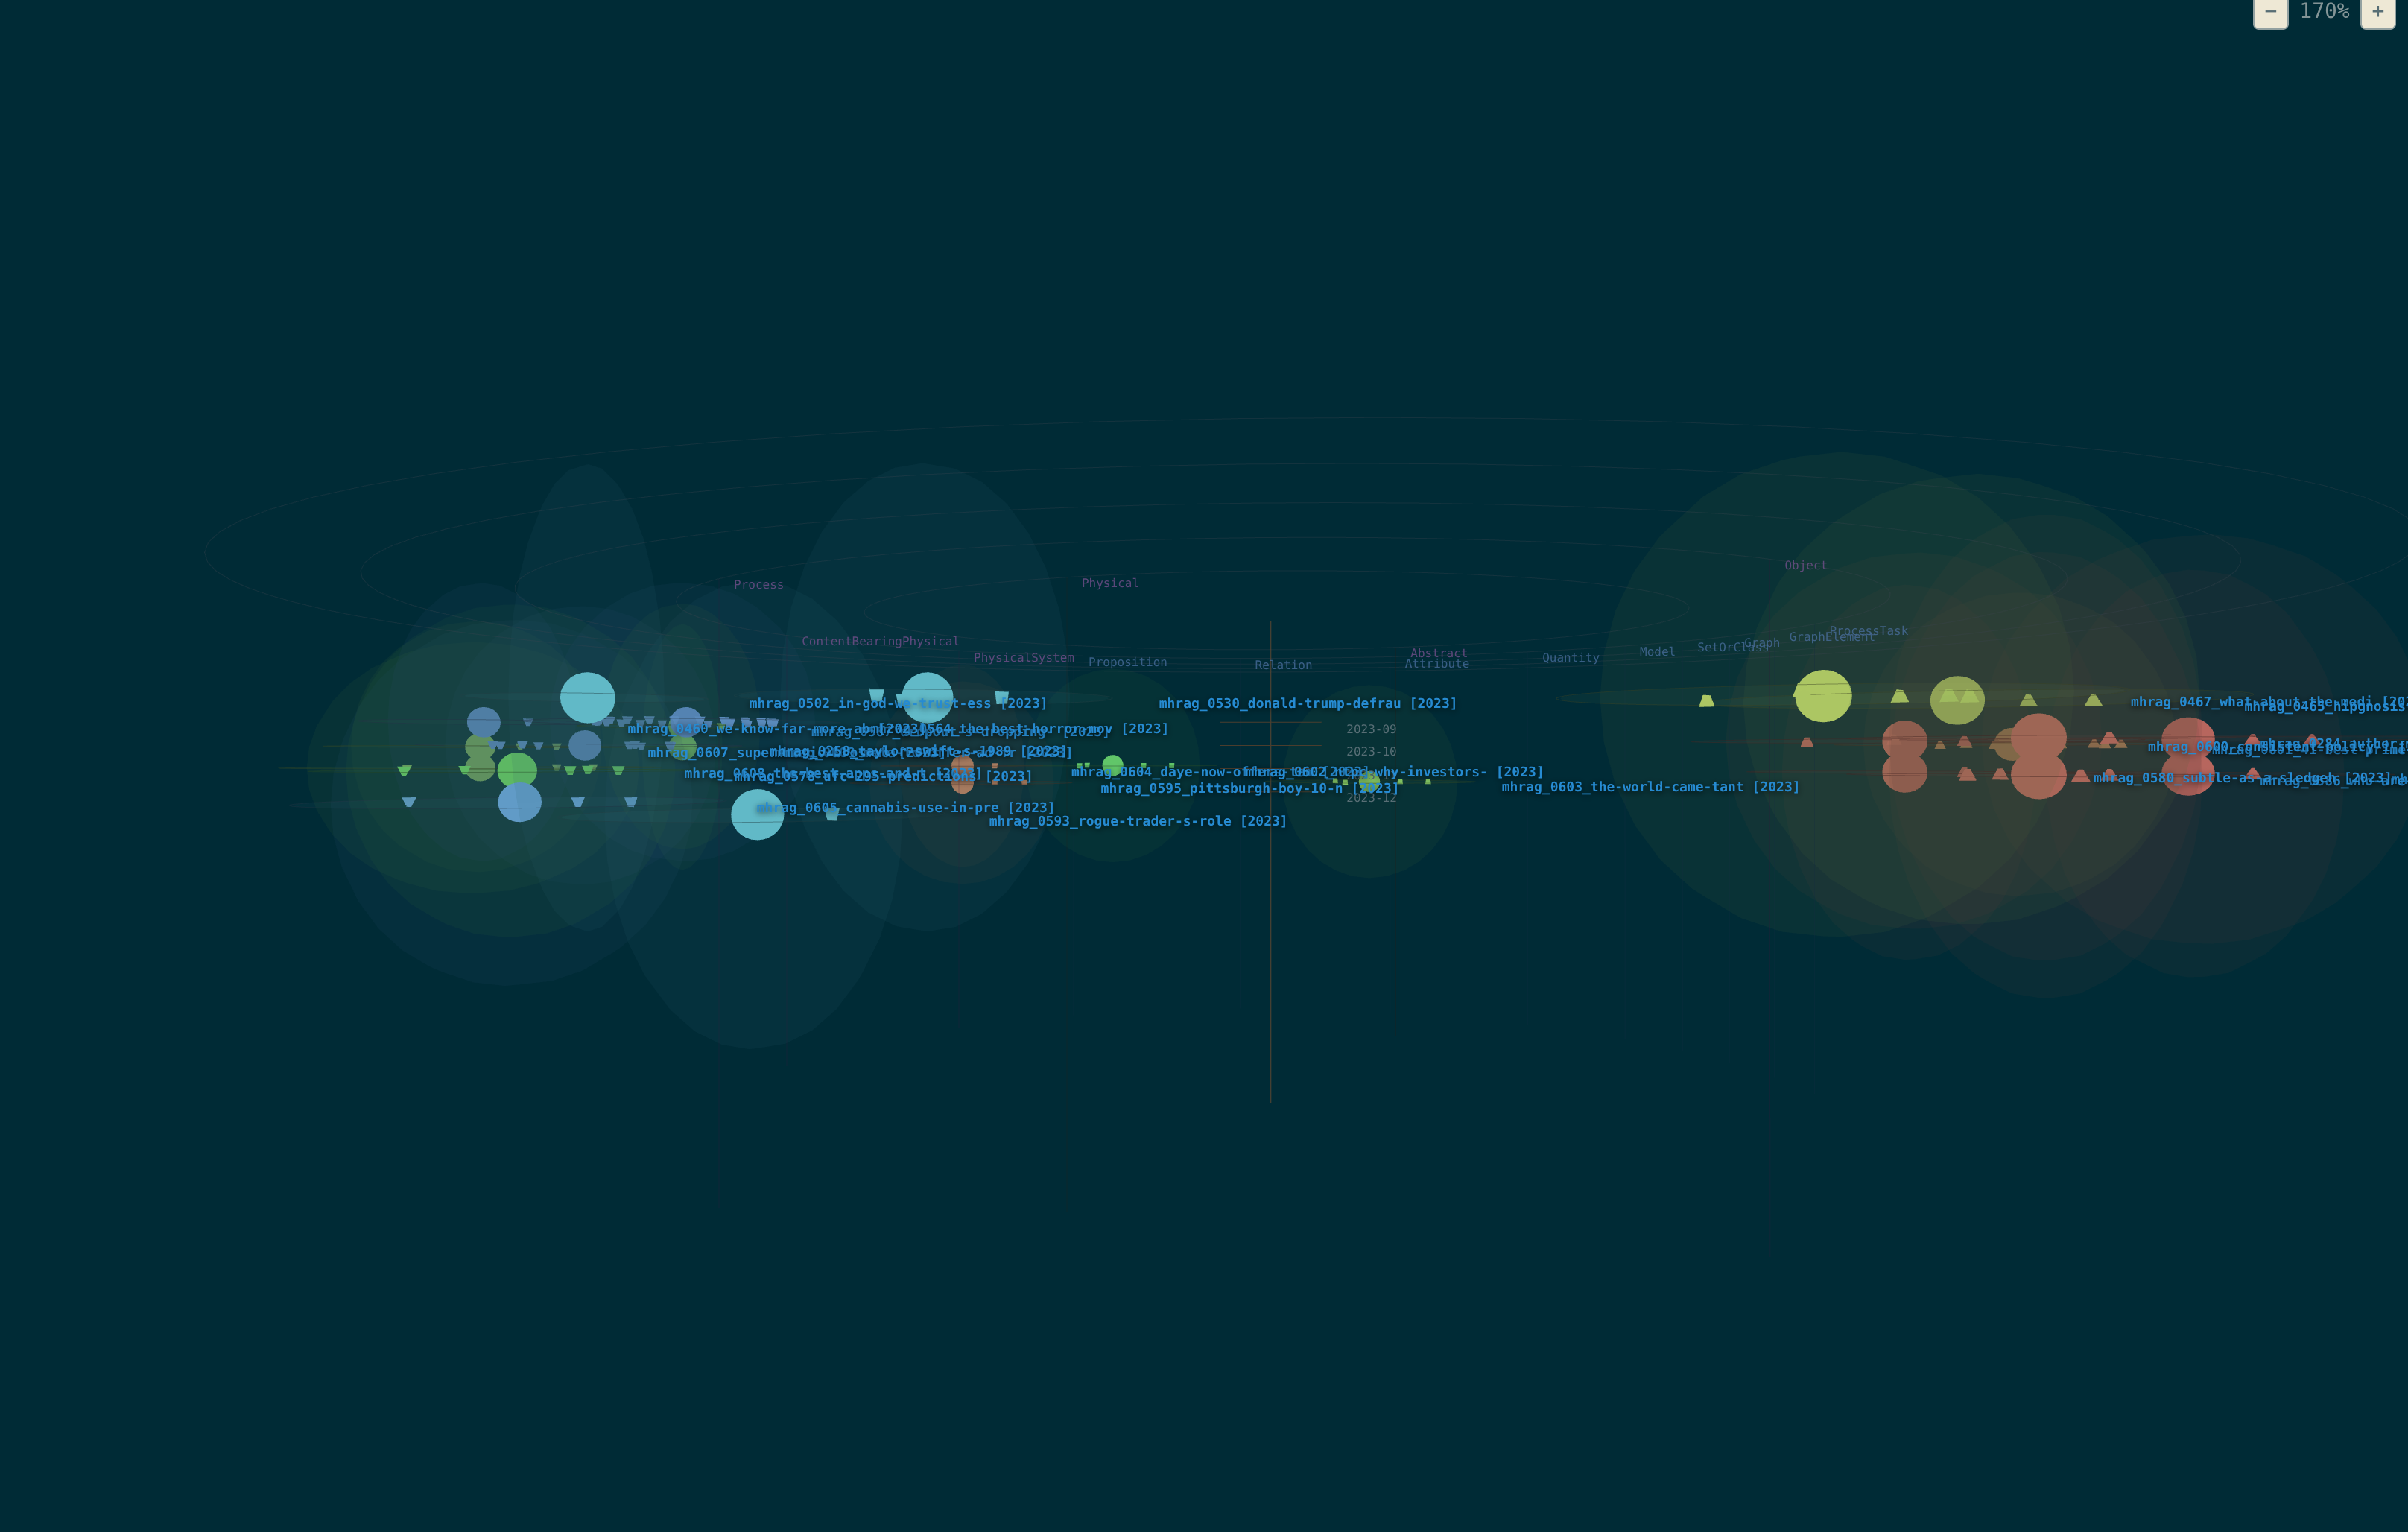
\includegraphics[width=0.48\columnwidth]{figs/sunburst_top.png}
\hfill
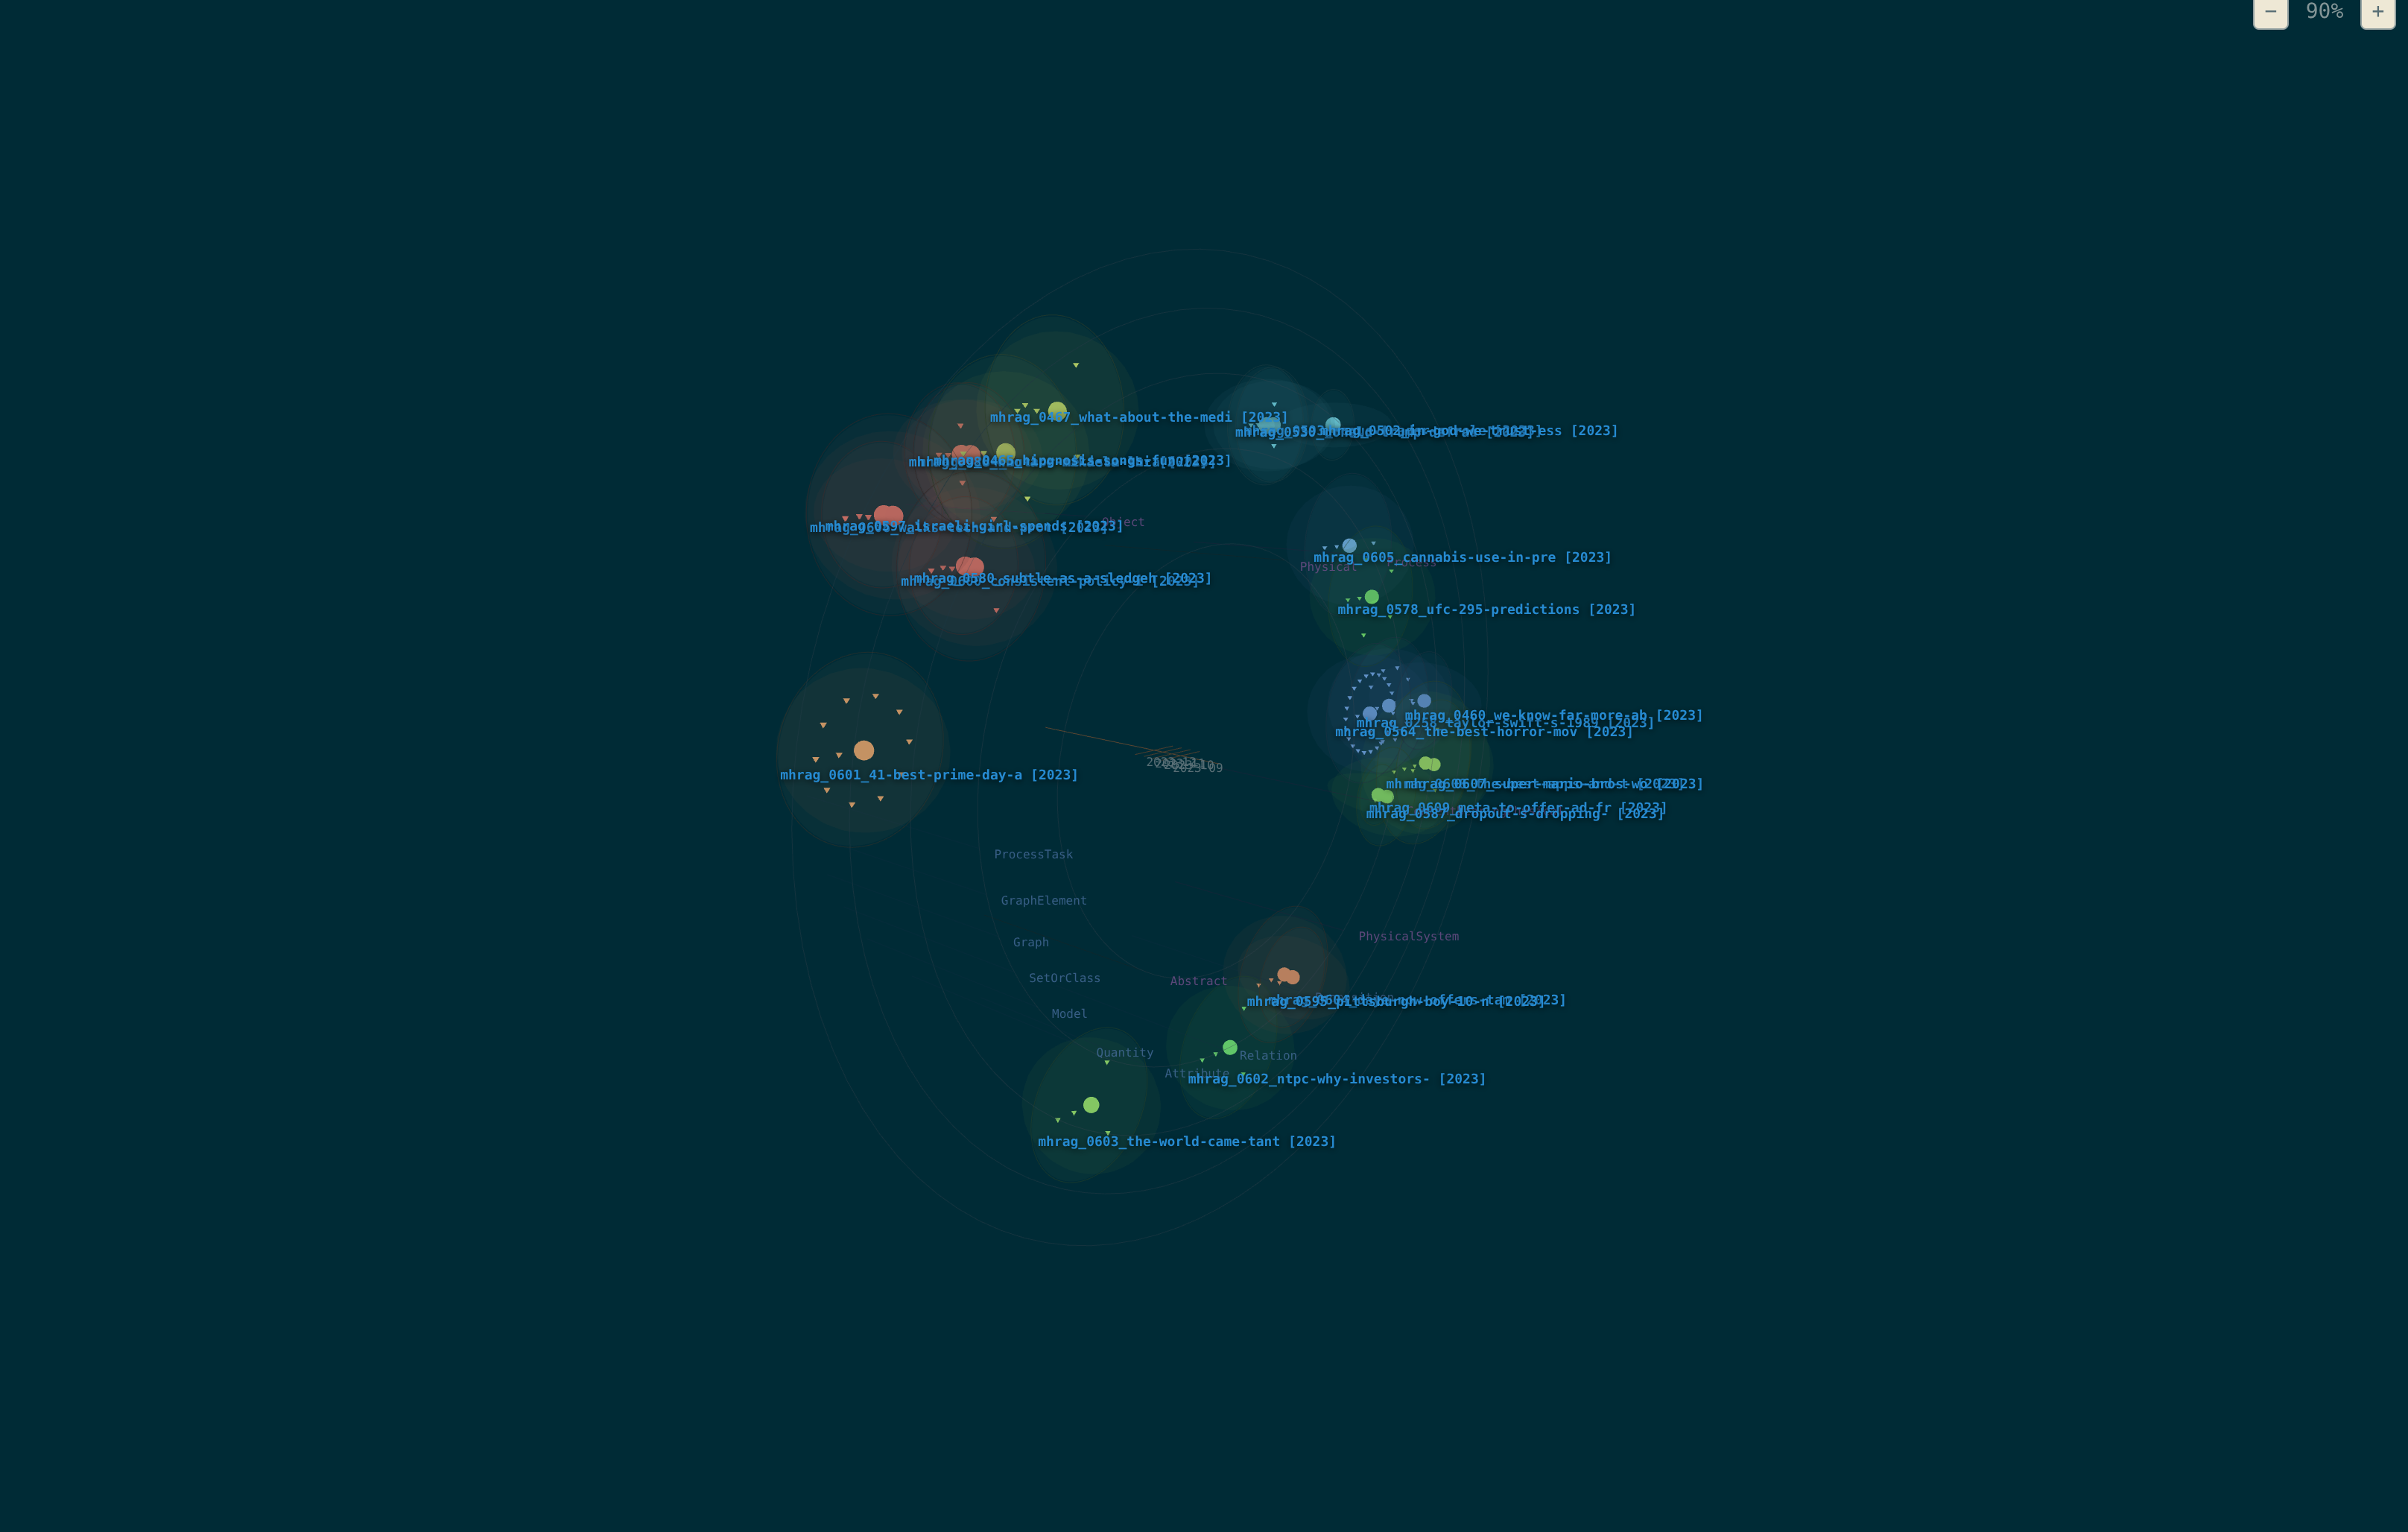
\includegraphics[width=0.48\columnwidth]{figs/tunnel_oblique.png}
\\[4pt]
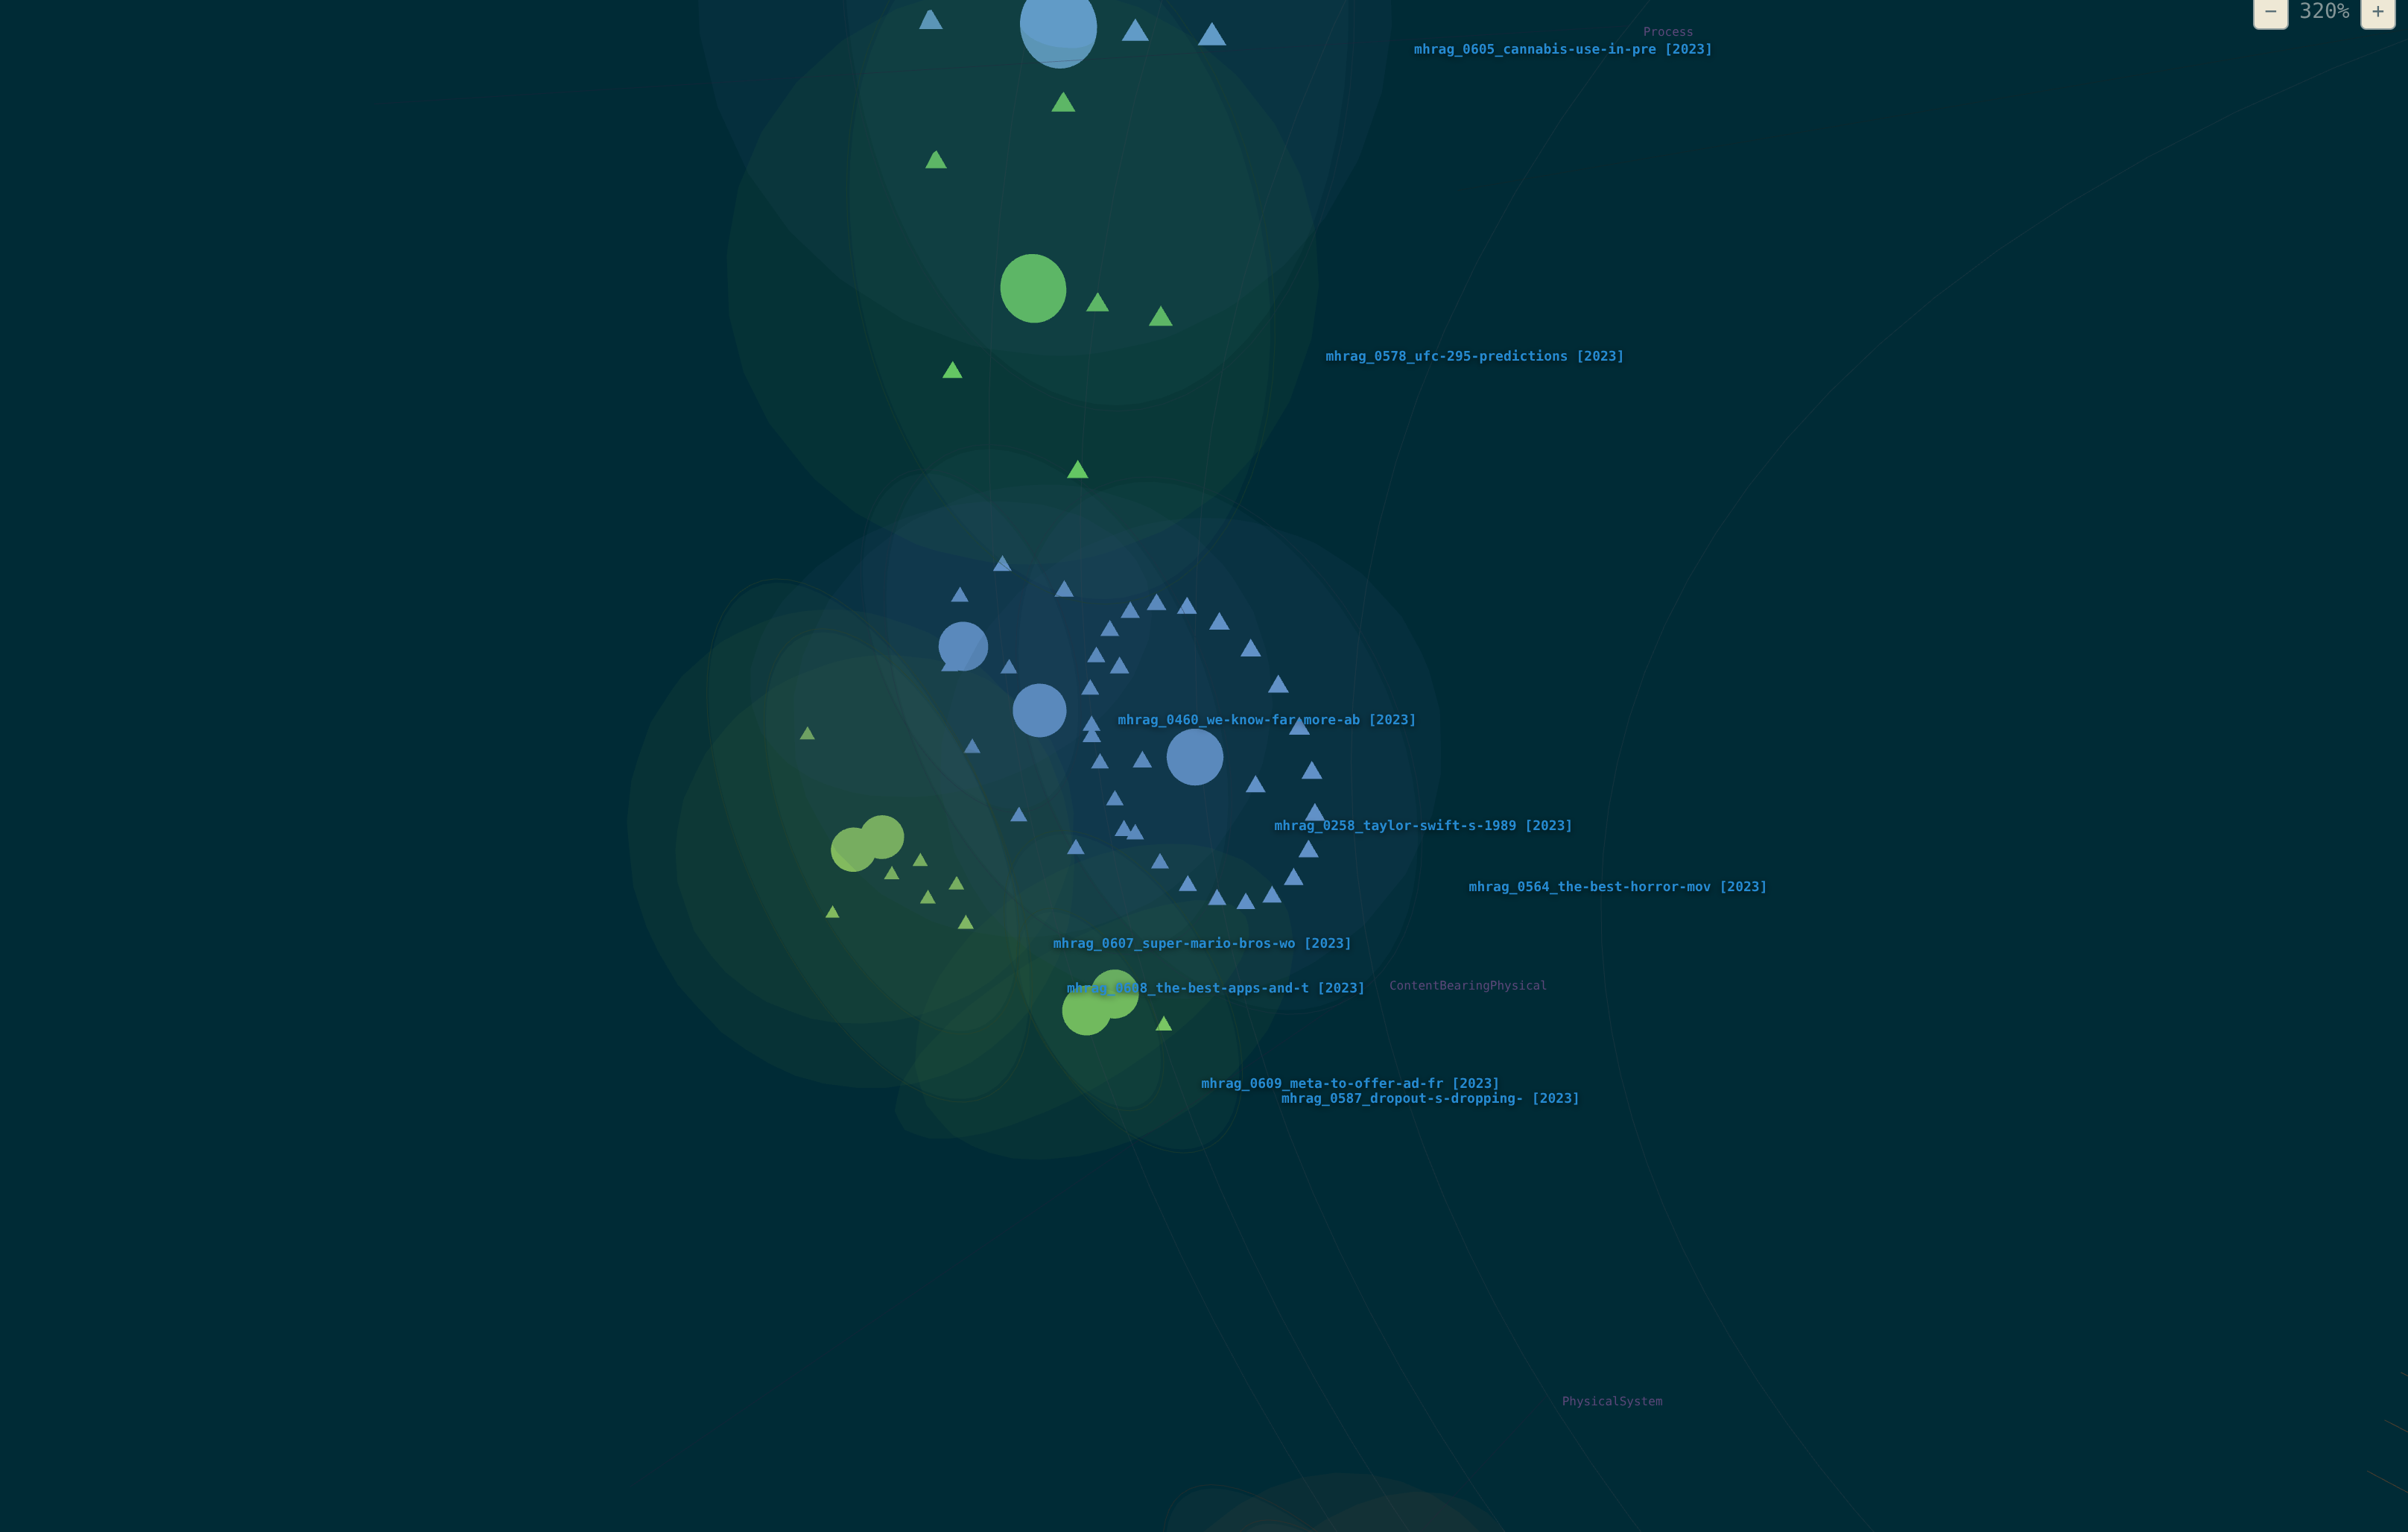
\includegraphics[width=0.7\columnwidth]{figs/disc_closeup.png}
\caption{Three camera views of the same 25-document Space-Time Graph (color = top SUMO category per document). \emph{Top left}: sunburst top-down, looking down $-$Y along the ontology cross-section -- documents cluster into SUMO category columns (\textit{Process}, \textit{Physical}, \textit{Object}, \textit{Proposition} labels visible). \emph{Top right}: oblique tunnel view, camera offset along Z so publication time reads as depth. \emph{Bottom}: close-up on a single document disc, showing its section hierarchy as a concentric ring of nodes (triangles) around the document root (sphere).}
\label{fig:viz}
\end{figure}

\section{Conclusion}

OHARA's Space-Time Graph -- structural hierarchy, temporal decay, and cross-document ontology unified in one substrate -- renders as a navigable 3D sunburst-tunnel and feeds a multi-phase retriever that delivers tiered, provenance-carrying results at parity with the best single-signal retriever, not superiority over it. The differentiated, quantitatively supported contribution is corroboration-gated abstention: a knowledge base that says ``I don't know'' on 45.6\% of unanswerable queries where a top-$k$ cut cannot, at no cost to Principal-hit rate on answerable ones. Ingest builds the full semantic graph at $\sim$\$12 per 1{,}000 documents; rendering scales sub-linearly. We frame this work as the opening of a research line: the substrate, harness, and honest ``not-yet'' results (Sec.~VII) are the foundation for the open hypotheses above.

\section*{Acknowledgments}
This research is supported by research funding from University of Science, Vietnam National University -- Ho Chi Minh City.

\begin{thebibliography}{9}

\bibitem{liu2024lost}
N.~F. Liu, K.~Lin, J.~Hewitt, A.~Paranjape, M.~Bevilacqua, F.~Petroni, and P.~Liang, ``Lost in the middle: How language models use long contexts,'' \emph{Trans. Assoc. Comput. Linguist.}, vol.~12, pp.~157--173, 2024.

\bibitem{stasko2000focus}
J.~Stasko and E.~Zhang, ``Focus+context display and navigation techniques for enhancing radial, space-filling hierarchy visualizations,'' in \emph{Proc. IEEE InfoVis}, 2000, pp.~57--65.

\bibitem{tang2024multihop}
Y.~Tang and Y.~Yang, ``MultiHop-RAG: Benchmarking retrieval-augmented generation for multi-hop queries,'' arXiv:2401.15391, 2024.

\bibitem{dasigi2021qasper}
P.~Dasigi, K.~Lo, I.~Beltagy, A.~Cohan, N.~A. Smith, and M.~Gardner, ``A dataset of information-seeking questions and answers anchored in research papers,'' in \emph{Proc. NAACL}, 2021, pp.~4599--4610.

\bibitem{gao2023ragsurvey}
Y.~Gao, Y.~Xiong, X.~Gao, K.~Jia, J.~Pan, Y.~Bi, Y.~Dai, J.~Sun, Q.~Guo, M.~Wang, and H.~Wang, ``Retrieval-augmented generation for large language models: A survey,'' arXiv:2312.10997, 2023.

\bibitem{peng2024graphrag_survey}
B.~Peng, Y.~Zhu, Y.~Liu, X.~Bo, H.~Shi, C.~Hong, Y.~Zhang, and S.~Tang, ``Graph retrieval-augmented generation: A survey,'' arXiv:2408.08921, 2024.

\bibitem{edge2024graphrag}
D.~Edge, H.~Trinh, N.~Cheng, J.~Bradley, A.~Chao, A.~Mody, S.~Truitt, and J.~Larson, ``From local to global: A graph RAG approach to query-focused summarization,'' arXiv:2404.16130, 2024.

\bibitem{guo2024lightrag}
Z.~Guo, L.~Xia, Y.~Yu, T.~Ao, and C.~Huang, ``LightRAG: Simple and fast retrieval-augmented generation,'' arXiv:2410.05779, 2024.

\bibitem{gutierrez2024hipporag}
B.~J. Gutierrez, Y.~Shu, Y.~Gu, M.~Yasunaga, and Y.~Su, ``HippoRAG: Neurobiologically inspired long-term memory for large language models,'' in \emph{Proc. NeurIPS}, 2024.

\bibitem{asai2023selfrag}
A.~Asai, Z.~Wu, Y.~Wang, A.~Sil, and H.~Hajishirzi, ``Self-RAG: Learning to retrieve, generate, and critique through self-reflection,'' in \emph{Proc. ICLR}, 2024.

\bibitem{yan2024crag}
S.-Q. Yan, J.-C. Gu, Y.~Zhu, and Z.-H. Ling, ``Corrective retrieval augmented generation,'' arXiv:2401.15884, 2024.

\end{thebibliography}

\end{document}
